\documentclass{thesisclass}
% Based on thesisclass.cls of Timo Rohrberg, 2009
% ----------------------------------------------------------------
% Thesis - Main document
% ----------------------------------------------------------------


%% ---------------------------------
%% | Information about the thesis  |
%% ---------------------------------

\newcommand{\myname}{Martin Thoma}
\newcommand{\mytitle}{On-line recognition of handwritten mathematical symbols}
\newcommand{\myinstitute}{Institute for Anthropomatics and Robotics (IAR)}  % TODO

\newcommand{\reviewerone}{Dr. St\"ucker} % TODO
\newcommand{\reviewertwo}{?} % TODO
\newcommand{\advisor}{Prof. Dr. Waibel}
\newcommand{\advisortwo}{Prof. Dr. Metze}

\newcommand{\timestart}{XX. Monat 2014} % TODO
\newcommand{\timeend}{XX. Monat 2014} % TODO
\newcommand{\submissiontime}{DD. MM. 2014} % TODO
\newcommand{\submissionplace}{Pittsburgh} % TODO

%% -------------------------------
%% |  Information for PDF file   |
%% -------------------------------
\hypersetup{
 pdfauthor={\myname},
 pdftitle={\mytitle},
 pdfsubject={Handwriting recognition}, % TODO
 pdfkeywords={Machine Learning} % TODO
}

%% ---------------------------------
%% | ToDo Marker - only for draft! |
%% ---------------------------------
% Remove this section for final version!
\setlength{\marginparwidth}{20mm}

\newcommand{\margtodo}
{\marginpar{\textbf{\textcolor{red}{ToDo}}}{}}

\newcommand{\todo}[1]
{{\textbf{\textcolor{red}{(\margtodo{}#1)}}}{}}


%% --------------------------------
%% | Old Marker - only for draft! |
%% --------------------------------
% Remove this section for final version!
\newenvironment{deprecated}
{\begin{color}{gray}}
{\end{color}}


%% --------------------------------
%% | Settings for word separation |
%% --------------------------------
% Help for separation:
% In german package the following hints are additionally available:
% "- = Additional separation
% "| = Suppress ligation and possible separation (e.g. Schaf"|fell)
% "~ = Hyphenation without separation (e.g. bergauf und "~ab)
% "= = Hyphenation with separation before and after
% "" = Separation without a hyphenation (e.g. und/""oder)

% Describe separation hints here:
\hyphenation{
% Pro-to-koll-in-stan-zen
% Ma-na-ge-ment  Netz-werk-ele-men-ten
% Netz-werk Netz-werk-re-ser-vie-rung
% Netz-werk-adap-ter Fein-ju-stier-ung
% Da-ten-strom-spe-zi-fi-ka-tion Pa-ket-rumpf
% Kon-troll-in-stanz
}


%% ------------------------
%% |    Including files   |
%% ------------------------
% Only files listed here will be included!
% Userful command for partially translating the document (for bug-fixing e.g.)
\includeonly{%
titlepage,
declaration,
acknowledgement,
introduction,
content,
evaluation,
conclusion,
appendix
}

%!TEX root = thesis.tex
%Term definitions
\newacronym{ANN}{ANN}{artificial neural network}
\newacronym{DTW}{DTW}{dynamic time warping}
\newacronym{MLP}{MLP}{multilayer perceptron}

% Term definitions
\newglossaryentry{epoch}{name={epoch}, description={During iterative training of a neural network, an \textit{epoch} is a single pass through the entire training set, followed by testing of the verification set.\cite{Concise12}}}

\newglossaryentry{learning rate}{name={learning rate}, description={A factor $0 \leq \eta \in \mdr$ that affects how fast new weights are learned. $\eta=0$ means that no new data is learned}, symbol={\ensuremath{\eta}}}

\newglossaryentry{learning rate decay}{name={learning rate decay}, description={The learning rate decay $0 < \alpha \leq 1$ is used to adjust the learning rate. After each epoch the learning rate $\eta$ is updated to $\eta \gets \eta \times \alpha$}, symbol={\ensuremath{\eta}}}

%%%%%%%%%%%%%%%%%%%%%%%%%%%%%%%%%
%% Here, main documents begins %%
%%%%%%%%%%%%%%%%%%%%%%%%%%%%%%%%%
\begin{document}
% Remove the following line for German text
\selectlanguage{english}

\frontmatter
\pagenumbering{roman}
%% titlepage.tex
%%

% coordinates for the bg shape on the titlepage
\newcommand{\diameter}{20}
\newcommand{\xone}{-15}
\newcommand{\xtwo}{160}
\newcommand{\yone}{15}
\newcommand{\ytwo}{-253}

\begin{titlepage}
% bg shape
\begin{tikzpicture}[overlay]
\draw[color=gray]  
 		 (\xone mm, \yone mm)
  -- (\xtwo mm, \yone mm)
 arc (90:0:\diameter pt) 
  -- (\xtwo mm + \diameter pt , \ytwo mm) 
	-- (\xone mm + \diameter pt , \ytwo mm)
 arc (270:180:\diameter pt)
	-- (\xone mm, \yone mm);
\end{tikzpicture}
    \begin{textblock}{10}[0,0](4,2.5)
        \includegraphics[width=.3\textwidth]{logos/KITLogo_RGB.pdf}
    \end{textblock}
    \begin{textblock}{10}[0,0](13,2.5)
        
\includegraphics[width=.3\textwidth]{logos/cmu-logo.pdf}
    \end{textblock}
	\changefont{phv}{m}{n}	% helvetica	
	\vspace*{3.5cm}
	\begin{center}
		\Huge{\mytitle}
		\vspace*{2cm}\\
		\Large{
			\iflanguage{english}{Bachelor's Thesis of}			
												  {Bachelorarbeit\\von}
		}\\
		\vspace*{1cm}
		\huge{\myname}\\
		\vspace*{1cm}
		\Large{
			\iflanguage{english}{At the Department of Informatics}			
													{An der Fakult\"at f\"ur Informatik}
			\\
			\myinstitute\\
            Karlsruhe Institute of Technology (KIT)\\
            Karlsruhe, Germany\\
		}
        \vspace*{1cm}
        \Large{
            \iflanguage{english}{School of Computer Science}            
                                                    {An der Fakult\"at f\"ur Informatik}
            \\
            Language Technologies Institute (LTI)\\ % TODO
            Carnegie Mellon University (CMU)\\
            Pittsburgh, United States
        }
	\end{center}
	\vspace*{0.5cm}
\Large{
\begin{center}
\begin{tabular}[ht]{l c l}
  % Gutachter sind die Professoren, die die Arbeit bewerten. 
  \iflanguage{english}{Reviewer}{Erstgutachter}: & \hfill  & \reviewerone\\
  \iflanguage{english}{Second reviewer}{Zweitgutachter}: & \hfill  & \reviewertwo\\
  \iflanguage{english}{Advisor}{Betreuender Mitarbeiter}: & \hfill  & \advisor\\
  \iflanguage{english}{Second advisor}{Zweiter betreuender Mitarbeiter}: & \hfill  & \advisortwo\\
  % Der zweite betreuende Mitarbeiter kann weggelassen werden. 
\end{tabular}
\end{center}
}


\vspace{2cm}
\begin{center}
\large{\iflanguage{english}{Duration}{Bearbeitungszeit}: \timestart \hspace*{0.25cm} -- \hspace*{0.25cm} \timeend}
\end{center}


\begin{textblock}{10}[0,0](4,16.8)
\tiny{ 
	\iflanguage{english}
		{KIT -- University of the State of Baden-Wuerttemberg and National Research Center of the Helmholtz Association}
		{KIT -- Universit\"at des Landes Baden-W\"urttemberg und nationales Forschungszentrum in der Helmholtz-Gemeinschaft}
}
\end{textblock}

\begin{textblock}{10}[0,0](14,16.75)
\large{
	\textbf{www.kit.edu} 
}
\end{textblock}

\end{titlepage}

\cleardoublepage
\vspace*{36\baselineskip}
\hbox to \textwidth{\hrulefill}
\par
\iflanguage{english}{I declare that I have developed and written the enclosed thesis completely by myself, and have not used sources or means without declaration in the text.}{Ich versichere wahrheitsgem\"a\ss, die Arbeit selbstst\"andig angefertigt, alle benutzten Hilfsmittel vollst\"andig und genau angegeben und alles kenntlich gemacht zu haben, was aus Arbeiten anderer unver\"andert oder mit Ab\"anderungen entnommen wurde.}

\textbf{\submissionplace, \submissiontime}
\vspace{1.5cm}

\dotfill\hspace*{8.0cm}\\
\hspace*{2cm}(\textbf{\myname}) %center name with hspace

\thispagestyle{empty}
%!TEX root = thesis.tex
\chapter*{Acknowledgement}

TODO

\begin{figure}[h]
    \centering
    \includegraphics*[width=0.5\linewidth, keepaspectratio]{logos/interact-logo.pdf} 
\end{figure}

\begin{figure}[h]
    \centering
    \includegraphics*[width=\linewidth, keepaspectratio]{logos/bw-stipendium.png} 
\end{figure}
\blankpage


%% -------------------
%% |   Directories   |
%% -------------------
\tableofcontents
\blankpage


%% -----------------
%% |   Main part   |
%% -----------------
\mainmatter
\pagenumbering{arabic}
%!TEX root = thesis.tex
\chapter{Introduction}\label{ch:Introduction}

Handwriting recognition is the task of finding a proper textual representation
given a handwritten symbol or sequence of symbols.

In off-line handwriting recognition, all algorithms have to work on pixel image
information of the handwriting. On-line handwriting recognition on the other
hand can use the information how symbols were written. This thesis is about
on-line handwriting recognition.


\section{Mathematical notation}

I will use the notation $v^{(i)}$ when I want to write about the $i$-th element
of a vector $v$. Vectors will always be denoted by lowercase latin letters.

Matrices will be denoted by uppercase latin letters.

The number of training examples will be denoted with $m$, the input vector with
$x$ and the output vector with $y$.

A single training example thus is given by the tuple $(x, y)$.

Parameters that are to be learned will be denoted with $\theta$.
%!TEX root = thesis.tex

%% ==============
\chapter{Baseline system} %TODO
\label{ch:Content1}
%% ==============

A system for symbol recognition was already written and is described in \cite{Kirsch}.


%% ===========================
\section{Section 1}
\label{ch:Content1:sec:Section1}
%% ===========================

\dots


%% ===========================
\section{Section 2}
\label{ch:Content1:sec:Section2}
%% ===========================

\dots


%% content.tex
%%

%% ==============
\chapter{Artificial Neural Nets}
\label{ch:Content2}
%% ==============

\Glspl{ANN} are models for classification that were inspired by the brain.
They consist of artificial neurons and have a lot of different subtypes like
Feed Forward Neural Nets.


%% ===========================
%!TEX root = thesis.tex
\section{Artificial neurons}\label{sec:artificial-neurons}
%% ===========================

Artificial neurons are inspired by biological neurons. Signals are send within 
the cell by charged particles, so called \textit{ions}. But before a biological
neuron sends a signal, a threshold charge has to be reached at the axon
hillock. This threshold charge is called \textit{action potential}. The action
potential can be reached by multiple factors, but the one I want to focus on
are charges send by other neurons. Depending on where the other axon terminals
are located and how long the distance to the axon hillock is, the signal contributes
more or less to reaching the action potential. After that, it simply sends a
signal.

\begin{figure}[ht]
    \centering
    \subfloat[Biological Neuron]{
        \includegraphics*[width=0.48\linewidth, keepaspectratio]{figures/biological-neuron.jpg} 
        \label{fig:biological-neuron}
    }%
    \subfloat[Artificial Neuron]{
        \resizebox{0.45\linewidth}{!}{\input{figures/artificial-neuron.tex}}
        \label{fig:artificial-neuron}
    }%
    \label{fig:artificial-and-biological-neuron}
    \caption{Both neurons receive weighted input, apply a function to that and give output}
\end{figure}

Artificial neurons are similar. They receive at least one input and give at
least one output. Those inputs might get weighted as well as the output.

The neurons apply a function to the sum of all weighted inputs. This function
is also called \textit{activation function}.

An artificial neuron using the unit step function (see \cref{f:unitstep}) is called
a \textit{perceptron}.


The artificial neuron sums all weighted inputs $x_i \cdot w_i$ up
             and applies its activation function $f$ to it.

%% ===========================
\section{Feedforward Neural Nets}
\label{ch:Content2:sec:Section2}
%% ===========================

Feedforward neural nets don't have loops.

\section{Activation functions}
\begin{figure}[ht]
    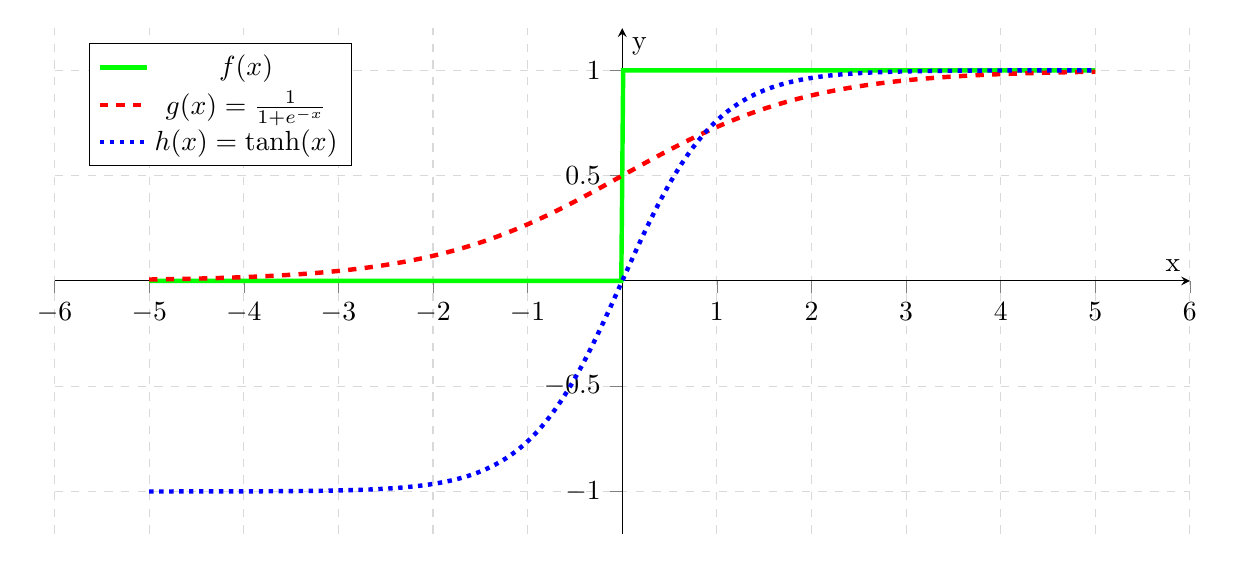
\begin{tikzpicture}[scale=1.0]
        \begin{axis}[
            legend pos=north west,
            axis x line=middle,
            axis y line=middle,
            grid = major,
            width=16cm,
            height=8cm,
            grid style={dashed, gray!30},
            xmin=-5,     % start the diagram at this x-coordinate
            xmax= 5,    % end   the diagram at this x-coordinate
            ymin=-1,     % start the diagram at this y-coordinate
            ymax= 1,   % end   the diagram at this y-coordinate
            %axis background/.style={fill=white},
            xlabel=x,
            ylabel=y,
            tick align=outside,
            enlargelimits=true]
          \addplot[domain=-5:5, green, ultra thick,samples=500] {x < 0 ? 0 : 1};
          \addplot[domain=-5:5, red, ultra thick,samples=500, dashed] {1/(1+exp(-x))};
          \addplot[domain=-5:5, blue, ultra thick,samples=500, dotted] {tanh(x)};
          \addlegendentry{$f(x)$} %TODO: \begin{cases} 0, & x < 0, \\ 1, & x \ge 0, \end{cases} (spacing)
          \addlegendentry{$g(x)=\frac{1}{1+e^{-x}}$}
          \addlegendentry{$h(x)=\tanh(x)$}
        \end{axis} 
    \end{tikzpicture}
    \caption{The unit step function $f$, the sigmoid function $g$ and the hyperbolic tangend $h$.}
    \label{fig:logistic-function}
\end{figure}

\subsection{Unit step function}\label{f:unitstep}


\subsection{Sigmoid function}\label{f:sigmoid}



\subsection{Hyperbolic tangent}\label{f:tanh}
%!TEX root = thesis.tex

\chapter{Evaluation}\label{ch:Evaluation}
A recognition system has two important characteristics: Its recognition accuracy
and the time it needs to recognize a new symbol. Recognition accuracy and time
are measured with new data which was not seen before.

Tests can be divided into two groups: Tests where some examples of the handwriting
of the writer were known at training time and tests were that's not the case.

Known-writer tests are created this way:

\begin{algorithm}[h]
    \begin{algorithmic}
        \State data $\gets k$-dimensional array of Lists
        \State $i \gets 0$
        \State Group labeled datasets by symbol
        \State Filter all symbols that have less than $k$ datasets
        \ForAll{Group $g$ in datasets}
            \ForAll{Dataset $(x, t)$ in $g$}
                \State data[$i$].$\Call{append}{(x, t)}$
                \State $i \gets (i + 1) \mod k$
            \EndFor
        \EndFor
    \end{algorithmic}
\caption{Creation of $k$ bins of datasets}
\label{alg:creation-of-bins}
\end{algorithm}

After that, a $k$-fold cross validation is run:

\begin{algorithm}[h]
    \begin{algorithmic}
        \Function{crossvalidation}{$k$, grouped dataset $d$, classificator $c$}
            \State correct, wrong $\gets 0, 0$
            \State c10, w10 $\gets 0, 0$
            \For{$i \in 0, \dots, k-1$}
                \For{$j \in 0, \dots, k-1$}
                    \If{$i \neq j$}
                        \State $c.\Call{train}{d[i]}$
                    \EndIf
                \EndFor
                \ForAll{$(x, t) \in d[i]$}
                    \Comment List of possible classifications descending by probability
                    \State $L \gets c.\Call{classify}{x}$
                    \If{$L[0] == t$}
                        \State correct $\gets$ correct $+1$
                        \State c10 $\gets$ c10 $+1$
                    \ElsIf{$t \in L$}
                        \State c10 $\gets$ c10 $+1$
                        \State wrong $\gets$ wrong $+1$
                    \Else
                        \State w10 $\gets$ wrong $+1$
                        \State wrong $\gets$ wrong $+1$
                    \EndIf
                \EndFor
            \EndFor
            \State \Return $(\frac{\text{correct}}{\text{correct}+\text{wrong}}, \frac{c10}{c10 + w10})$
        \EndFunction
    \end{algorithmic}
\caption{$k$-fold cross-validaton}
\label{alg:k-fold-cross-validation}
\end{algorithm}

I will call result of such a 10-fold cross-validation
\textit{classification accuracy}. The first part of the tupel is called \textit{Top-1 accuractiy}
and the second one is called \textit{Top-10 accuracy}.

\section{Baseline system: Greedy matching}
The greedy matching algorithm got with scaling and shifting (see \cpageref{alg:scale-and-shift})
a Top-1 accuracy of 83.11\% and a Top-10 accuracy of 97.66\%.
%!TEX root = thesis.tex

\chapter{Conclusion}\label{ch:Conclusion}

\dots



%% --------------------
%% |   Bibliography   |
%% --------------------
\cleardoublepage
\phantomsection
\addcontentsline{toc}{chapter}{\bibname}

\iflanguage{english}
{\bibliographystyle{IEEEtranSA}}	% english style %TODO 'An hmm-smm...'
{\bibliographystyle{babalpha-fl}}	% german style
												  
% Use IEEEtran for numeric references
%\bibliographystyle{IEEEtranSA})

\bibliography{thesis}

\printglossaries

%% ----------------
%% |   Appendix   |
%% ----------------
\cleardoublepage

%!TEX root = thesis.tex

%% ==============================
%\chapter{Appendix}
%\label{ch:Appendix}
%% ==============================

\appendix

\iflanguage{english}
{\addchap{Appendix}}	% english style
{\addchap{Anhang}}	% german style


\section{Algorithms}\label{appendix:algorithms}
\begin{algorithm}[h]
  \begin{algorithmic}
    \State $a \gets \text{next from}~A$
    \State $b \gets \text{next from}~B$
    \State $d \gets \delta(a,b)$
    \State $a' \gets \text{next from}~A$
    \State $b' \gets \text{next from}~B$
    \While{points left in $A$ $\wedge$ points left in $B$}
      \State $l, m, r \gets \delta(a',b), \delta(a', b'), \delta(a, b')$
      \State $\mu \gets \min ~\{l, m, r\}$
      %\COMMENT{ Important line }
      \State $d \gets d + \mu$
      \If{$l = \mu$}
        \State $a \gets a'$
        \State $a' \gets \text{next from}~A$
      \ElsIf{$r = \mu$}
        \State $b \gets b'$
        \State $b' \gets \text{next from}~B$
      \Else
        \State $a \gets a'$
        \State $b \gets b'$
        \State $a' \gets \text{next from}~A$
        \State $b' \gets \text{next from}~B$
      \EndIf
    \EndWhile
    \If{no points left in $A$}
      \ForAll{points $p$ in $B$}
        \State $d \gets d + \delta(a',p)$
      \EndFor
    \ElsIf{no points left in $B$}
      \ForAll{points $p$ in $A$}
        \State $d \gets d + \delta(b',p)$
      \EndFor
    \EndIf
  \end{algorithmic}
  \caption{Greedy matching as described in \cite{Kirsch}}
  \label{alg:greedy-matching}
\end{algorithm}

\begin{algorithm}[h]
    \begin{algorithmic}
        \Function{scale\_and\_shift}{$pointlist$}
            \State $min_x, min_y = pointlist[0]['x'], pointlist[0]['y']$
            \State $max_x, max_y = pointlist[0]['x'], pointlist[0]['y']$
            \ForAll{$lines$ in $pointlist$}
                \ForAll{$p$ in $lines$}
                    \If{$p['x'] < min_x$}
                        \State $min_x \gets p['x']$
                    \ElsIf{$p['x'] > max_x$}
                        \State $max_x \gets p['x']$
                    \EndIf

                    \If{$p['y'] < min_y$}
                        \State $min_y \gets p['y']$
                    \ElsIf{$p['y'] > max_y$}
                        \State $max_y \gets p['y']$
                    \EndIf
                \EndFor
            \EndFor

            \State $width, height \gets max_x - min_x, max_y - min_y$

            \State $factor = 1$

            \If{$width \neq 0$}
                \State $factor_x = \frac{1}{width}$
            \EndIf

            \If{$height \neq 0$}
                \State $factor_y = \frac{1}{height}$
            \EndIf

            \State $factor = \min(factor_x, factor_y)$
            \State $add_x, add_y = 0, 0$

            \ForAll{$lines$ in $pointlist$}
                \ForAll{$p$ in $lines$}
                    \State $p['x'] \gets (p["x"] - minx) \cdot factor$
                    \State $p['y'] \gets (p["y"] - miny) \cdot factor$
                \EndFor
            \EndFor

            \Return $pointlist$
        \EndFunction
    \end{algorithmic}
\caption{Scale and shift a list of lines to the $(0,1) \times (0, 1)$ unit square}
\label{alg:scale-and-shift}
\end{algorithm}

\section{Figures}\label{appendix:figures}
\setcounter{figure}{0}
% TODO
\begin{figure} [ht]
    \centering
    ein Bild
    \caption{A figure}
    \label{fig:BPMNBeispiela}
\end{figure}


\end{document}
